
\subsection{Flowchart of Methodology}
The following flowchart illustrates the steps involved in developing the spell-correcting chatbot:
\begin{figure}[h!]
    \centering
    \documentclass{standalone}
\usepackage{tikz}
\usetikzlibrary{shapes.geometric, arrows}

\tikzstyle{startstop} = [rectangle, rounded corners, minimum width=3cm, minimum height=1cm, text centered, draw=black, fill=red!30]
\tikzstyle{process} = [rectangle, minimum width=3cm, minimum height=1cm, text centered, draw=black, fill=orange!30]
\tikzstyle{arrow} = [thick,->,>=stealth]

\begin{document}

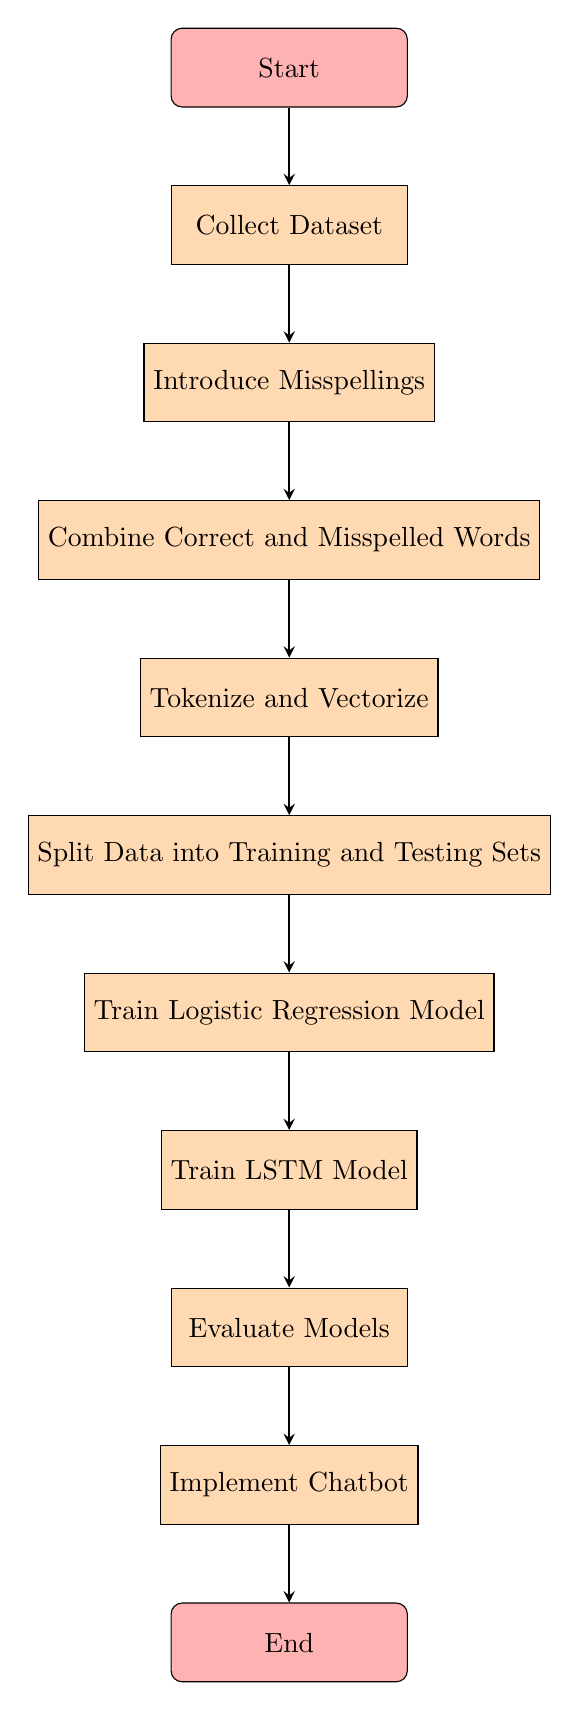
\begin{tikzpicture}[node distance=2cm]

\node (start) [startstop] {Start};
\node (collect) [process, below of=start] {Collect Dataset};
\node (introduce) [process, below of=collect] {Introduce Misspellings};
\node (combine) [process, below of=introduce] {Combine Correct and Misspelled Words};
\node (tokenize) [process, below of=combine] {Tokenize and Vectorize};
\node (split) [process, below of=tokenize] {Split Data into Training and Testing Sets};
\node (logreg) [process, below of=split] {Train Logistic Regression Model};
\node (lstm) [process, below of=logreg] {Train LSTM Model};
\node (evaluate) [process, below of=lstm] {Evaluate Models};
\node (chatbot) [process, below of=evaluate] {Implement Chatbot};
\node (end) [startstop, below of=chatbot] {End};

\draw [arrow] (start) -- (collect);
\draw [arrow] (collect) -- (introduce);
\draw [arrow] (introduce) -- (combine);
\draw [arrow] (combine) -- (tokenize);
\draw [arrow] (tokenize) -- (split);
\draw [arrow] (split) -- (logreg);
\draw [arrow] (logreg) -- (lstm);
\draw [arrow] (lstm) -- (evaluate);
\draw [arrow] (evaluate) -- (chatbot);
\draw [arrow] (chatbot) -- (end);

\end{tikzpicture}

\end{document}

    \caption{Flowchart of the methodology for developing the spell-correcting chatbot.}
    \label{fig:flowchart}
\end{figure}

\subsection{Data Collection and Preprocessing}
The first step in developing the spell-correcting chatbot was to collect and preprocess the data. I utilized the words corpus from the Natural Language Toolkit (NLTK), which contains a comprehensive list of English words. This dataset provided the foundation for both correctly spelled words and misspelled variants.

\subsubsection{Introducing Misspellings}
To simulate real-world scenarios where users may input misspelled words, I created a function to introduce random misspellings into the dataset. This function, introduce_misspellings, modifies a given word by randomly replacing one of its characters with another character from the alphabet, based on a specified error rate. The experimented error rates were 0.1(10\%), 0.5(50\%), and 0.8(80\%). This process generated a diverse set of misspelled words to train the model effectively.
\begin{lstlisting}[language=Python, caption=Data Collection and Preprocessing]
    import nltk
    from nltk.corpus import words
    import random
    
    # Download the dataset if not already done
    nltk.download('words')
    
    # Load the dataset
    word_list = words.words()
    
    # Function to introduce misspellings
    def introduce_misspellings(word, error_rate=0.1):
        if random.random() < error_rate:
            index = random.randint(0, len(word) - 1)
            return word[:index] + random.choice('abcdefghijklmnopqrstuvwxyz') + word[index + 1:]
        return word
    
    # Create a dataset with misspellings
    misspelled_word_list = [introduce_misspellings(word) for word in word_list]
    
\end{lstlisting}

\subsubsection{Combining Correct and Misspelled Words}
I combined the original correctly spelled words with the newly generated misspelled words to create a comprehensive dataset. Each word in the dataset was labeled as either correct (0) or misspelled (1).
\begin{lstlisting}[language=Python, caption=Data Collection and Preprocessing]
    # Combine correct and misspelled words
    combined_word_list = word_list + misspelled_word_list
    labels = [0] * len(word_list) + [1] * len(misspelled_word_list)    
\end{lstlisting}

\subsection{Tokenization and Vectorization}
To prepare the data for training, I used tokenization and vectorization techniques. Tokenization involved breaking down the words into individual characters, which were then converted into sequences of numerical values using the Keras Tokenizer. These sequences were padded to ensure uniform length, facilitating input into the neural network.

\subsection{Data Splitting}
The dataset was split into training and testing sets, with 80\% of the data used for training and 20\% reserved for testing. This ensured that the model was evaluated on data it had not seen during training, providing an accurate measure of its performance.

\subsection{Logistic Regression Model}
Initially, I implemented a Logistic Regression model with a pipeline using the 'liblinear' solver. This model served as a baseline to compare the performance with the more complex LSTM-based neural network.
\begin{lstlisting}[language=Python, caption=Data Collection and Preprocessing]
    from sklearn.preprocessing import StandardScaler
    from sklearn.pipeline import Pipeline
    from sklearn.model_selection import train_test_split
    from sklearn.linear_model import LogisticRegression
    from sklearn.metrics import accuracy_score, classification_report
    
    # Split the data
    X_train, X_test, y_train, y_test = train_test_split(X, labels, test_size=0.2, random_state=42)
    
    # Create a pipeline with scaling and logistic regression using 'liblinear' solver
    pipeline = Pipeline([
        ('scaler', StandardScaler(with_mean=False)),  # Scaling the data
        ('logreg', LogisticRegression(max_iter=1000, solver='liblinear'))  # Use 'liblinear' solver
    ])
    
    # Train the model
    pipeline.fit(X_train, y_train)
    
    # Evaluate the model
    y_pred = pipeline.predict(X_test)
    print(f"Accuracy: {accuracy_score(y_test, y_pred)}")
    print(classification_report(y_test, y_pred))
\end{lstlisting}


\subsection{LSTM-Based Neural Network Model}
To optimize and improve the accuracy, I built an LSTM-based neural network model according to Dhankhar(2018)\cite{DhanLSTM}. The model architecture consisted of an embedding layer, two LSTM layers, and a dense output layer with a sigmoid activation function.

¥begin{itemize}
    ¥item Embedding Layer: Converts the input sequences into dense vectors of fixed size.
    ¥item LSTM Layers: Capture the sequential dependencies in the character sequences.
    ¥item Dense Output Layer: Provides a binary classification output (correct or misspelled).
¥end{itemize}

\begin{lstlisting}[language=Python, caption=Data Collection and Preprocessing]
    from keras.models import Sequential
    from keras.layers import Embedding, LSTM, Dense
    
    # Build LSTM model
    model = Sequential()
    model.add(Embedding(input_dim=len(tokenizer.word_index) + 1, output_dim=50, input_length=max_seq_length))
    model.add(LSTM(100, return_sequences=True))
    model.add(LSTM(100))
    model.add(Dense(1, activation='sigmoid'))
    
    # Compile the model
    model.compile(optimizer='adam', loss='binary_crossentropy', metrics=['accuracy'])
    
\end{lstlisting}

\subsection{Training and Evaluation}
I experimented and turned with different hyperparameters, such as the error rate for generating misspellings, the number of epochs, and the batch size, to find the optimal configuration for the LSTM model. The final model was trained for 10 epochs with a batch size of 64 using error rate 0.8(80\%). The validation dataset was used to monitor the model's performance during training. After training, the model's accuracy was evaluated on the test dataset.
\begin{lstlisting}[language=Python, caption=Data Collection and Preprocessing]
    # Train the model
    history = model.fit(X_train, y_train, epochs=10, batch_size=64, validation_data=(X_test, y_test))
    
    # Evaluate the model
    loss, accuracy = model.evaluate(X_test, y_test)
    print(f"LSTM Model Accuracy: {accuracy}")
    
    # Predict and evaluate
    y_pred = (model.predict(X_test) > 0.5).astype("int32")
    print(f"LSTM Model Accuracy: {accuracy_score(y_test, y_pred)}")
    print(classification_report(y_test, y_pred))
    
\end{lstlisting}

\subsection{Chatbot Implementation}
The chatbot function was designed to take user input, preprocess it, and use the trained model to predict whether the input word was correctly spelled or not. If the word is misspelled, the chatbot suggest the most similar correctly spelled word based on character similarity and also displayed its matching accuracy. If the word is spelled correctly, the chatbot return "Nothing Wrong!".
\begin{lstlisting}[language=Python, caption=Data Collection and Preprocessing]
    # Chatbot function to correct spelling
    def correct_spelling(input_word):
        input_seq = tokenizer.texts_to_sequences([input_word])
        input_seq = pad_sequences(input_seq, maxlen=max_seq_length)
        
        prediction = model.predict(input_seq)
        
        if prediction < 0.5:
            return "Nothing Wrong!"
        
        # Find the most similar word
        similarities = []
        for word in word_list:
            if len(word) == len(input_word):
                sim = sum(1 for a, b in zip(word, input_word) if a == b)
                similarities.append((word, sim))
        if not similarities:
            return "No suggestions available."
        
        best_match = max(similarities, key=lambda x: x[1])[0]
        accuracy = max(similarities, key=lambda x: x[1])[1] / len(input_word) * 100
        
        return f"Suggested Correction: {best_match}, Matching Accuracy: {accuracy:.2f}%"
    
    # Simple chatbot interface
    def chatbot():
        print("Welcome to the English Correcting Chatbot! Type 'exit' to quit.")
        while True:
            user_input = input("Enter a word: ").strip()
            if user_input.lower() == 'exit':
                break
            correction = correct_spelling(user_input)
            print(correction)
    
    # Run the chatbot
    chatbot()
    
\end{lstlisting}

